\begin{figure}[H]
    \centering
    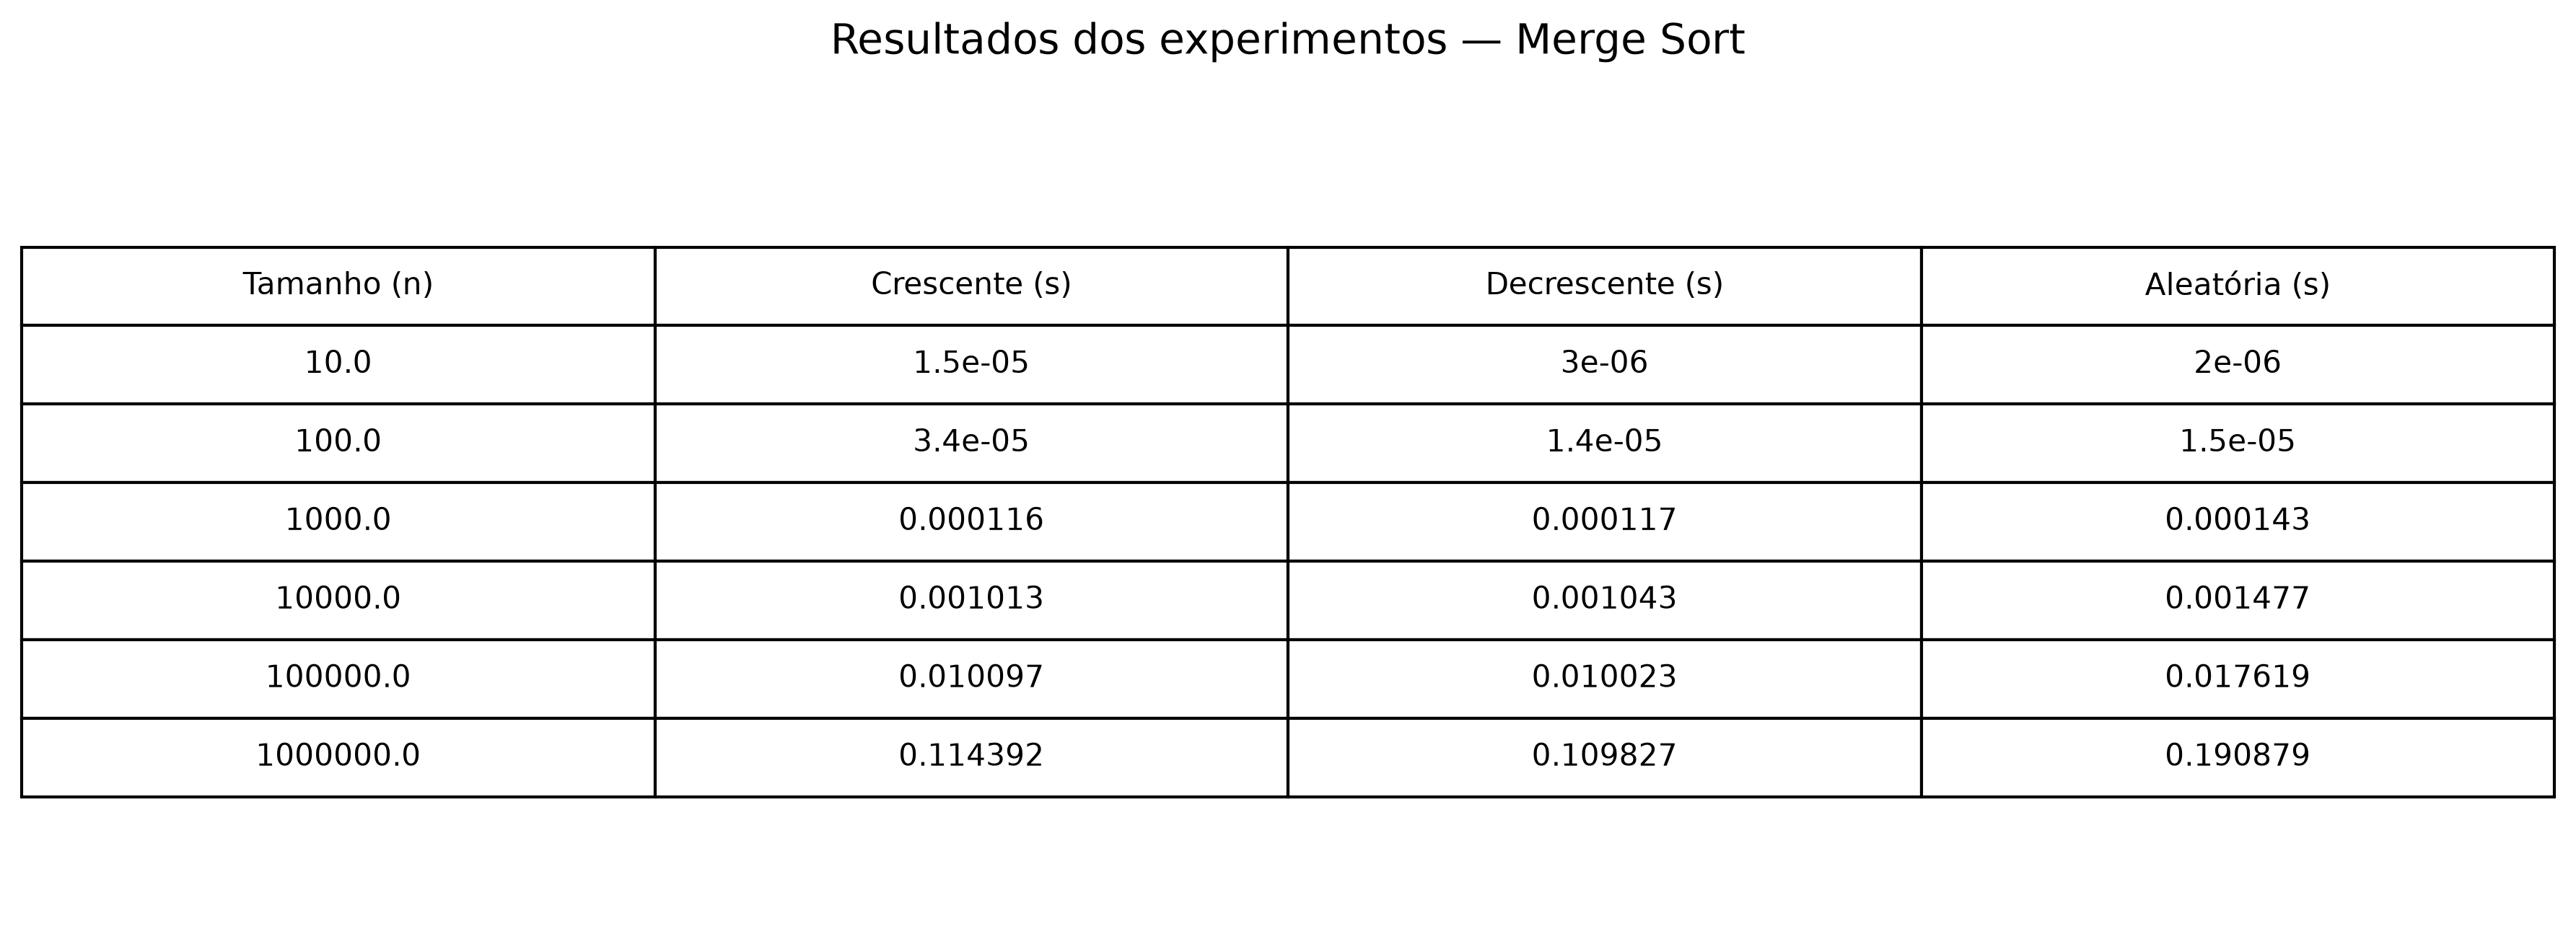
\includegraphics[width=16cm]{Imagens/Merge_Sort/tabela.png}
    \caption{Tabela de tempo de execução do algoritmo Merge Sort}
    \label{fig:tabela-merge}
\end{figure}

\begin{figure}[H]
    \centering
    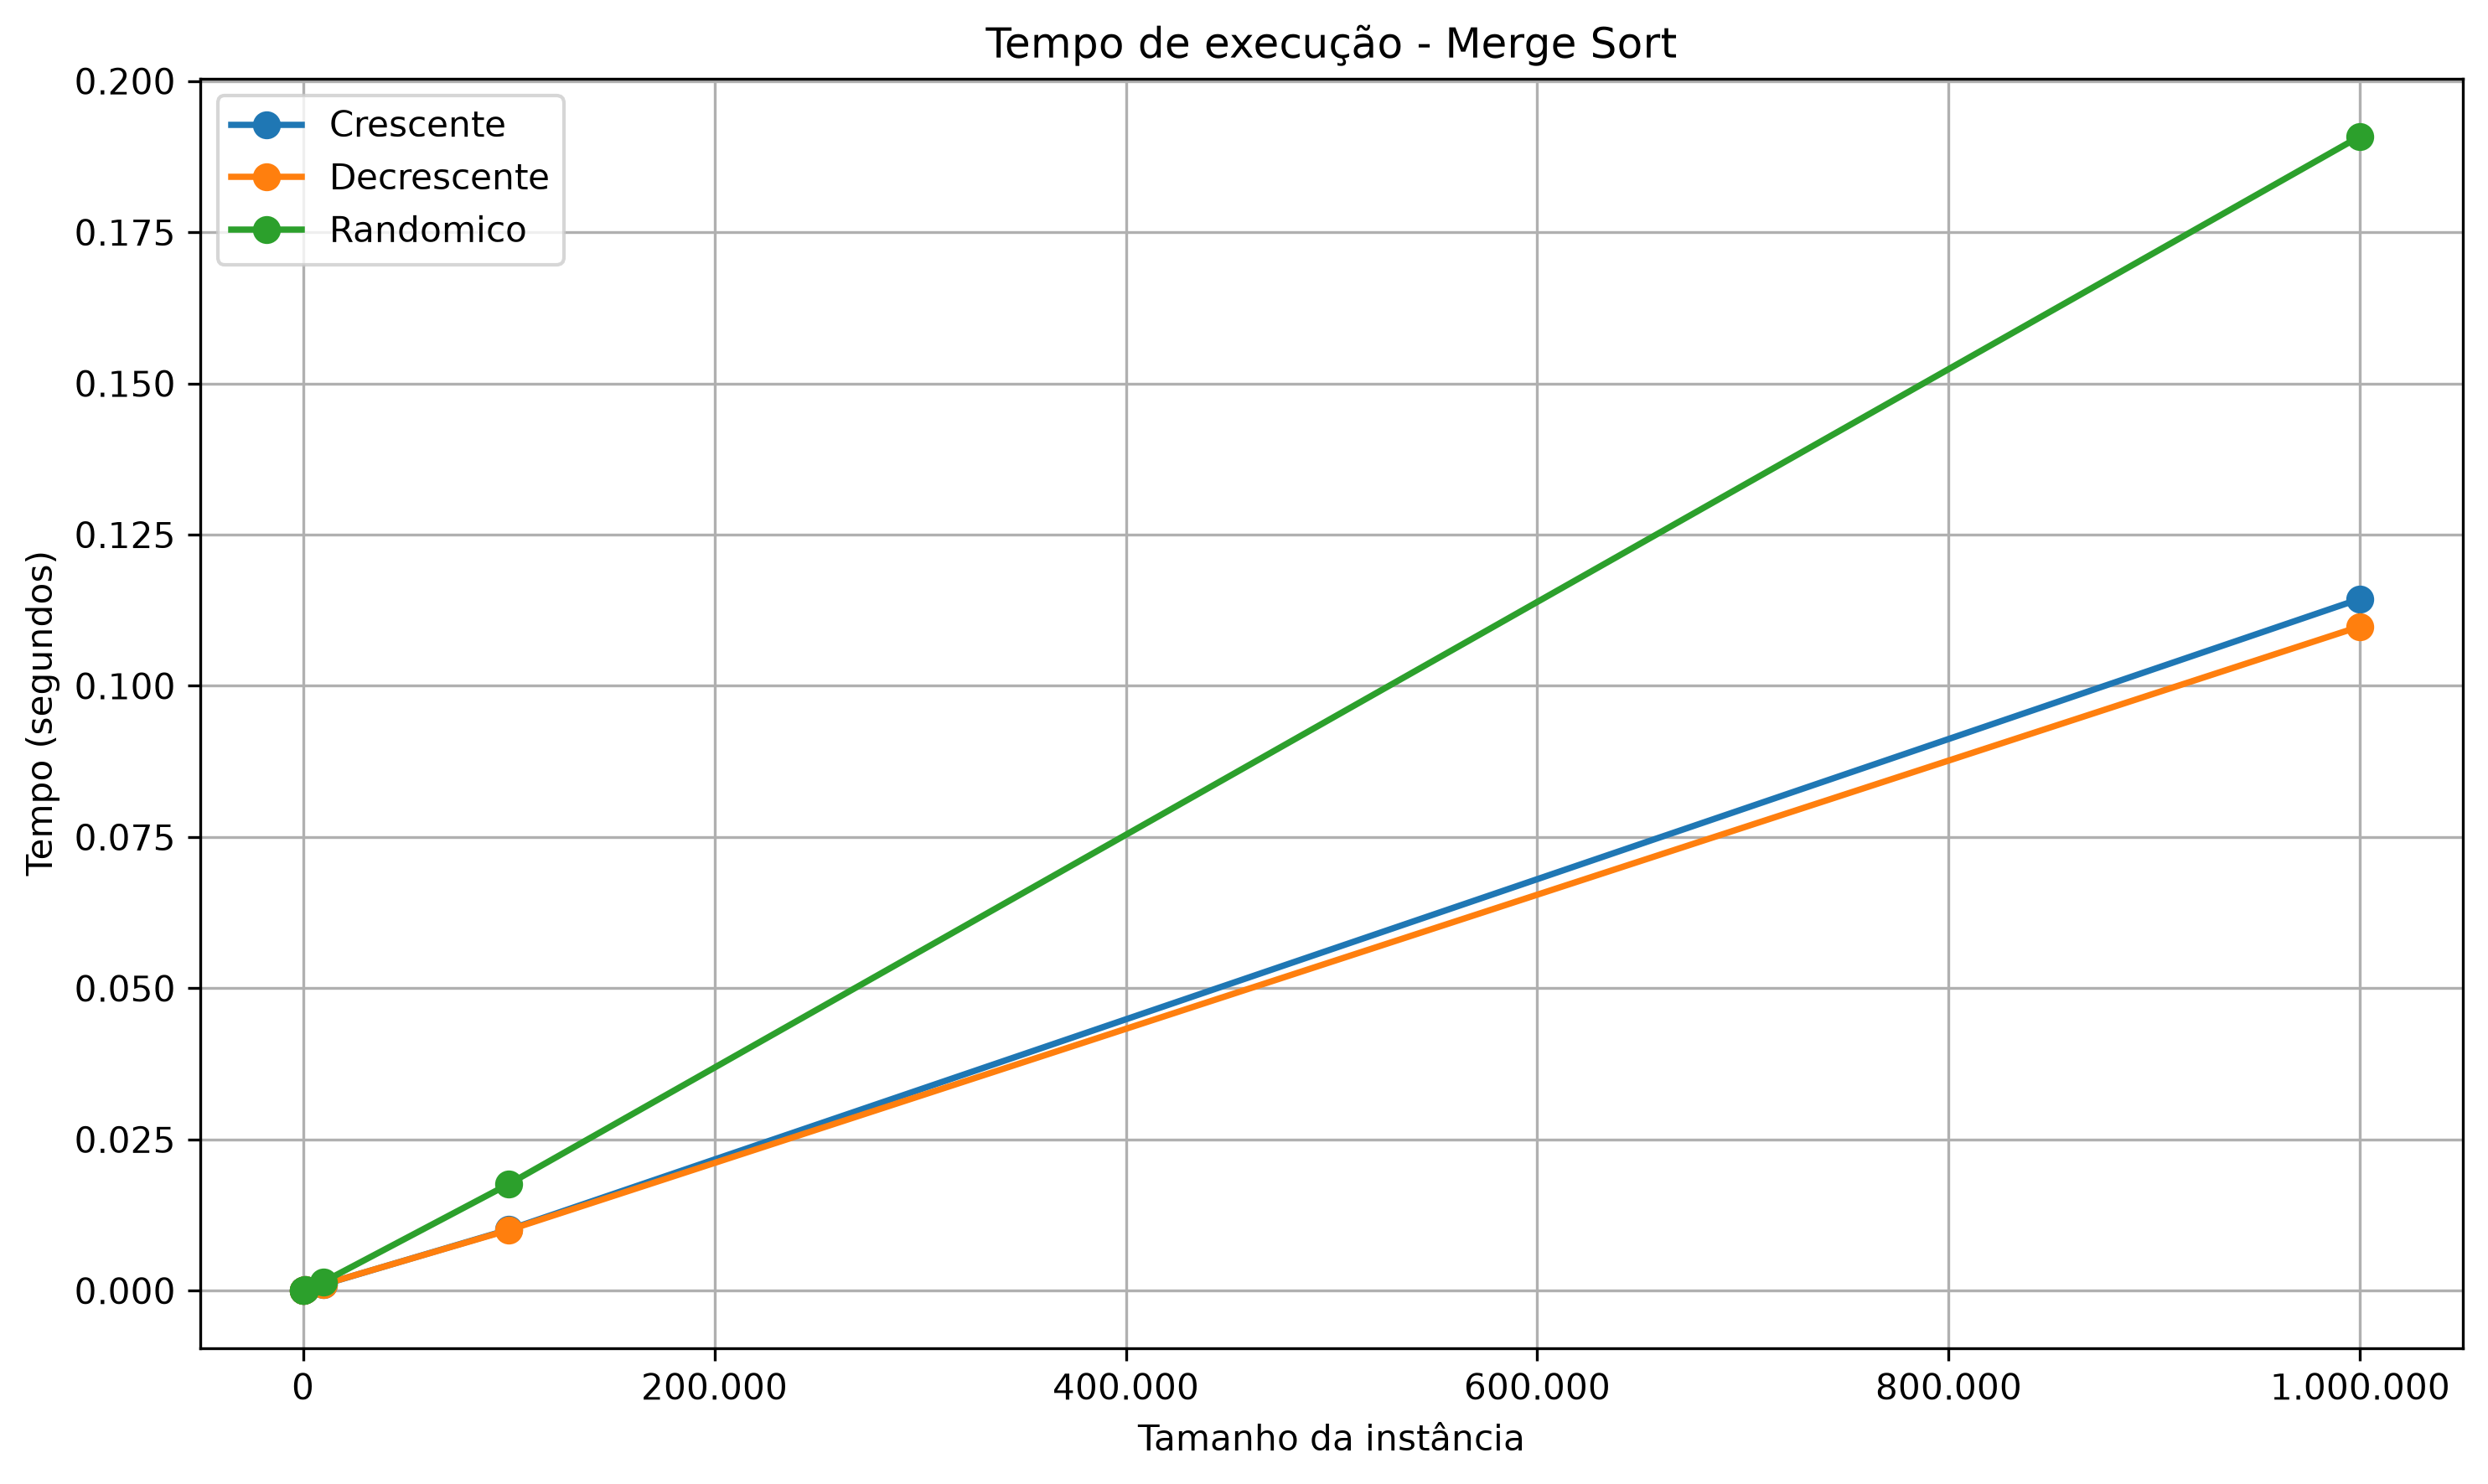
\includegraphics[width=10cm]{Imagens/Merge_Sort/grafico.png}
    \caption{Gráfico de tempo de execução do algoritmo Merge Sort}
    \label{fig:grafico-merge}
\end{figure}

Os resultados obtidos nos experimentos estão apresentados na tabela e no
gráfico. Observa-se que o algoritmo Merge Sort apresenta comportamento
semelhante para as entradas crescentes, decrescentes e aleatórias, pois
sua estratégia de divisão e conquista não depende significativamente
da organização inicial dos elementos.

Durante a execução, o vetor é dividido recursivamente em partes menores
e, posteriormente, essas partes são intercaladas em ordem crescente.
Como todos os elementos precisam ser processados durante as etapas de
intercalação, o algoritmo apresenta complexidade temporal
$\Theta(n\log n)$ nos casos analisados.

Os resultados também permitem observar que o aumento do tamanho da
entrada provoca um crescimento no tempo de execução. Entretanto, esse
crescimento tende a ser menos acentuado do que o observado nos algoritmos
com complexidade quadrática, especialmente para vetores de grandes
dimensões.

Além disso, a implementação utiliza vetores auxiliares durante a
intercalação dos elementos, necessitando de memória adicional
proporcional ao tamanho da entrada. Dessa forma, o Merge Sort apresenta
um bom desempenho para grandes conjuntos de dados, embora utilize mais
memória auxiliar do que algoritmos como o Insertion Sort.
